Since the scope of this project is different to the aim of most OMR applications, a lot of research was done into the current techniques used. Indeed, since the work spans several decades, computing power and technology have changed significantly and so many techniques have evolved, each suitable for different OMR purposes.

\section {\cite{taubman2005musichand}}

Taubman attempts to improve on notation input for professional musicians, allowing them to input rough ``sketched'' music and convert it into another musical format. The solution makes use of a graphics tablet connected to a desktop machine and records individual strokes the user makes.

Strokes are captured individually but using a latency threshold which is then used to group them together. Taubman then makes use of statistical moments \todo{Reference to Moments Tech background} to classify these stroke groups, making use of a K-NN classification algorithm.

The application also makes use of a great deal of domain expertise, since strokes are generally sketched as seen in \ref{fig:taubman-sketch}

\begin{figure}[h!]
  \frame{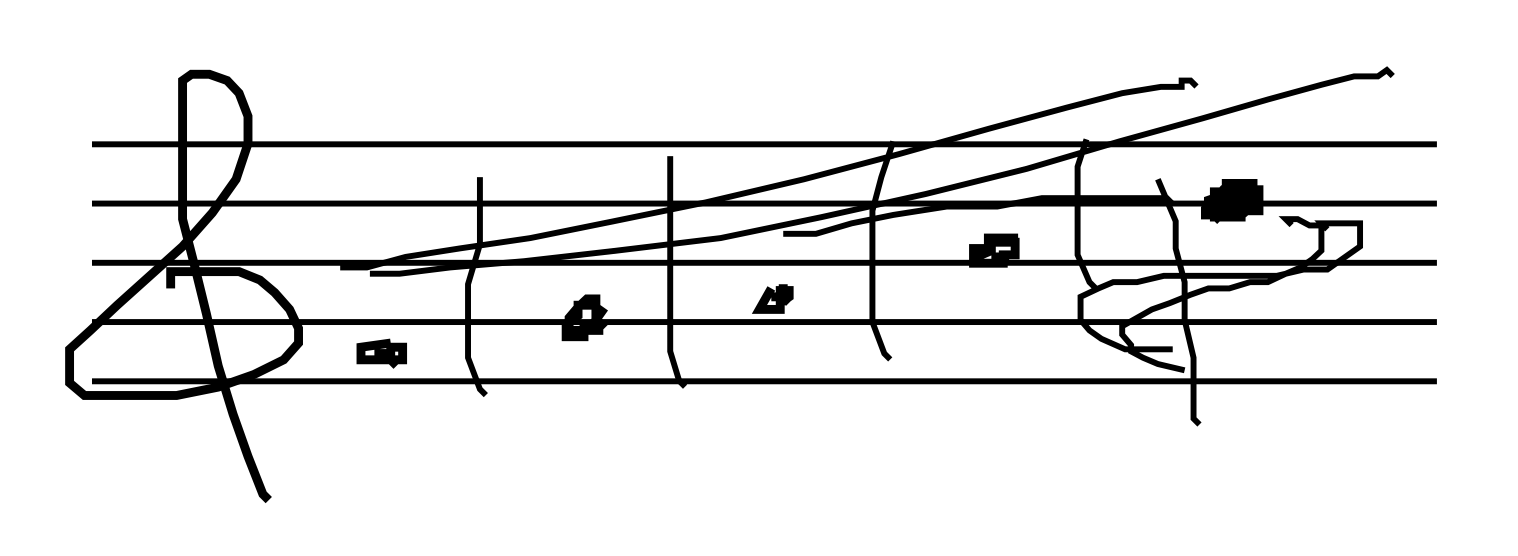
\includegraphics[width=\linewidth]{gfx/prior-research/taubman-sketch.png}}
  \centering
  \caption{Example notation sketch from \cite{taubman2005musichand}}
  \label{fig:taubman-sketch}
\end{figure}
